\documentclass[a4paper, 12pt]{article}
% math symbols
\usepackage{amssymb}
\usepackage{amsmath}
\usepackage{mathrsfs}
\usepackage{physsummer}


\usepackage{enumitem}
\usepackage[margin = 2cm]{geometry}

\tolerance = 1000
\emergencystretch = 0.74cm



\pagestyle{empty}
\parindent = 0mm

\begin{document}

\begin{center}
  \Large{\textbf{Городской центр физического образования, 10 класс.}\\
  \textit{Серия 21${}^{\ast}$, 2 апреля 2015.}}
\end{center}

\begin{center}
  \Large\textbf{ Повторение электростатики. }
\end{center}

\taskpic{ В электрической цепи, состоящей из идеального источника с
  ЭДС $\mathcal{E}$, двух конденсаторов с емкостями $2C$ и $C$ и
  резистора с некоторым сопротивлением, замыкают ключ \textbf{K1}. До
  каких напряжений зарядятся конденсаторы? 2) После того как
  конденсаторы полностью зарядились, замыкают ключ \textbf{K2} и
  размыкают его тогда, когда сила тока через источник уменьшается в 2
  раза по сравнению с силой тока через него сразу после замыкания
  ключа \textbf{K2}. Найдите количество теплоты $Q$, выделившееся в
  цепи за время, прошедшее с момента замыкания ключа \textbf{K2} до
  момента его размыкания. }
{
  \begin{tikzpicture}[circuit ee IEC, thick]
    \node[contact] (1) at (0,0) {}; \node[contact] (2) at (0,-2) {};
    \draw (1) to[capacitor={info'={$C$}}] (2) to[make
    contact={info'={\textbf{K2}}}] ++(right:1cm) to[resistor]
    ++(up:2cm) -- (1) to[capacitor={info'={$2C$}}] ++(left:2cm); \draw
    (2) to[make contact={info={\textbf{K1}}}] ++(left:2cm)
    to[battery] ++(up:2cm);
  \end{tikzpicture}
}

\taskpic{ В горизонтально расположенный плоский конденсатор до
  середины вставлен брусок, который может скользить без трения между
  пластинами конденсатора. Конденсатор подключен к источнику
  постоянного напряжения $U$. В некоторый момент времени брусок без
  толчка отпускают. Найдите зависимость скорости бруска $v$ от времени
  и постройте ее график. Геометрические размеры бруска
  $b \times b \times d$, его диэлектрическая проницаемость $\vareps$,
  плотность $\rho$. Расстояние между пластинами конденсатора $d$, их
  размеры $b \times b$.  }
{
  \begin{tikzpicture}
    \draw[line width=0.2cm] (0,0) -- (1.5,0);
    \draw[line width=0.2cm] (0,-1) -- (1.5,-1);
    \draw[fill=gray!20] (-1,-0.1) rectangle (1,-0.9);
    \draw[thick,<->,blue] (-0.8,-0.1) -- (-0.8,-0.9)
    node[right,midway] {$d$};
    \draw[very thick,-o] (1,0) -- ++(up:0.5cm) -- ++(right:0.8cm)
    --++(down:0.7cm);
    \draw[very thick,-o] (1,-1) -- ++(down:0.5cm) -- ++(right:0.8cm)
    --++(up:0.7cm);
    \draw (2,-0.5) node[blue] {$U$}; 
  \end{tikzpicture}
}

\taskpic[6cm]{ Стабилизированный источник тока способен выдавать постоянный
  ток $I_0$ независимо от подключённой к нему нагрузки. Источник включён
  в цепь. Все элементы цепи можно считать идеальными, их параметры
  указаны на рисунке. До замыкания ключа конденсатор не был заряжен. В
  некоторый момент времени ключ замкнули. Какое количество теплоты $Q$
  выделилось на резисторе $R$ после замыкания ключа? }
{
  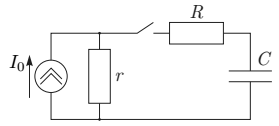
\includegraphics[width=6cm]{ru2014104.png}
}

\end{document}


%%% Local Variables: 
%%% mode: latex
%%% TeX-engine:xetex
%%% TeX-PDF-mode: t
%%% End:
